\section{Declustering}

It is generally assumed that the seismicity of each tectonic seismic source follows a Poissonian occurrence process. Therefore, in order to accomplish this, we declustered the earthquake catalog. In compiling the catalog of events, foreshocks and aftershocks were removed using a declustering methodology \citep{Gardner1974}. Fig.~\ref{fig:instrumental} shows the epicenter of declustered instrumental  earthquakes.

\begin{figure} [H]
\centering
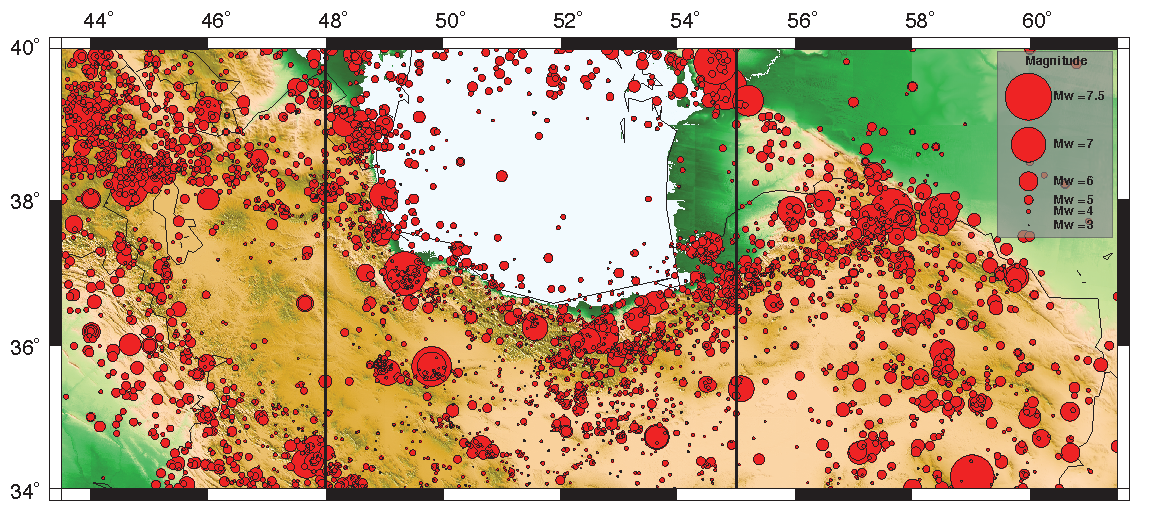
\includegraphics[scale=0.8]{figures/pdf/Figure3.pdf} 
\caption{Declustered instrumental seismicity map (after 1900) of Northern Iran. The study areas are separated at longitude of 48$^{\circ}$ and 55$^{\circ}$ . } 
\label{fig:instrumental}
\end{figure}




